\documentclass[11pt]{article}
\usepackage[width=7.0in, height=10.0in]{geometry}
\usepackage{hyperref}
\usepackage{amsmath}
\usepackage{upgreek}
\usepackage{bm}
\usepackage{mathtools}
\usepackage{tikz}
\usetikzlibrary{arrows}



\newcommand{\vct}[1]{\boldsymbol{\mathbf{#1}}}
\newcommand{\vr}{\vct{r}}
\newcommand{\vrN}{\vr^N}
\newcommand{\vrn}{\vr^n}
\newcommand{\dvr}{\frac{ d \vr  }{(2\pi)^3}}
\newcommand{\vx}{\vct{x}}
\newcommand{\vxN}{\vx^N}
\newcommand{\vxn}{\vx^n}
\newcommand{\dvx}{\frac{ d \vx  }{(2\pi)^3}}
\newcommand{\vk}{\vct{k}}
\newcommand{\dvk}{\frac{ d \vk  }{(2\pi)^3}}
\newcommand{\vy}{\vct{y}}
\newcommand{\vz}{\vct{z}}
\newcommand{\vE}{\vct{E}}
\newcommand{\vD}{\vct{D}}
\newcommand{\vP}{\vct{P}}
\newcommand{\vM}{\vct{M}}
\newcommand{\vMbar}{\overline{\vct{M}}}
\newcommand{\vdel}{\vct{\updelta}}
\newcommand{\vmu}{\vct{\upmu}}

\renewcommand{\theequation}{\thesection.\arabic{equation}}



\begin{document}


\title{Kirkwood's formula for the dielectric constant}
\author{ \vspace{-10ex} }
\date{ \vspace{-10ex} }
\maketitle


This note tries to explain the Kirkwood's 1939 paper\cite{kirkwood1939a}
on the dielectric constant.
%




\section{Technical notes on the Appendix}



\subsection{Kirkwood's three-tier model}



Kirkwood used a three-tier model.


The first tier is the molecule itself,
which carries a dipole of moment $\vmu$.
%
We assume that $\vmu$ is fixed,
and study how this fixed dipole polarize its surroundings.


The second tier is a sphere of radius $r_0$,
this sphere includes the molecule and its immediate neighbors.
%
The material within this sphere assumes a dielectric constant
much different from the macroscopic one $\epsilon$.
%
The total dipole moment of this sphere,
caused by the polarization of $\vmu$,
is given by $\vMbar(R, r_0)$.


The third tier is the entire dielectric,
which also assumes a spherical shape with radius $R$.
%
The total dipole moment of this largest sphere,
as a result of the polarization field of $\vmu$
is given by $\vMbar$.
%
The region between the second and third tiers
assume the macroscopic dielectric constant $\epsilon$.




%To model the cause of the dipole, $\vmu^*$,
%we consider an external field, $\vE_0$,
%which is defined as follows.
%%
%In vacuum,
%the molecule is polarized to have a dipole moment $\vmu^*$
%under $\vE_0$.
%
%
%From a distance $r \gg R$,
%the entire medium looks like a dipole of moment $\vMbar$.
%%
%According to Eq. \eqref{eq:Eplug},
%\begin{align*}
%%  \frac{ \vMbar } { 4 \pi \epsilon_0 }
%%&=
%%  \frac{ ( \epsilon - 1 ) \, R^3 } { \epsilon + 2 } \vE_0
%%\\
%  \vE_2
%&=
%  \frac{ 3 } { \epsilon + 2 } \vE_0.
%\end{align*}
%%
%Try to argue
%$E_2 \cdot \vmu^* = E_0 \cdot \vMbar$.
%Then
%\begin{equation}
%  \vMbar
%=
%  \frac{ 3 } { \epsilon + 2 } \vmu^*
%\end{equation}
%
%According to Eq. \eqref{eq:Ehole},
%\begin{align*}
%  \vE^*
%&=
%  \frac{ 3 \epsilon } { 2 \epsilon + 1 } \vE_1.
%\end{align*}
%Try to argue
%$E_1 \cdot \vmu^* = E^* \cdot \vMbar$.
%Then
%\begin{equation}
%  \vmu^*
%=
%  \frac{ 3 \epsilon } { 2 \epsilon + 1}
%  \vMbar(R, r_0).
%\end{equation}



\begin{center}
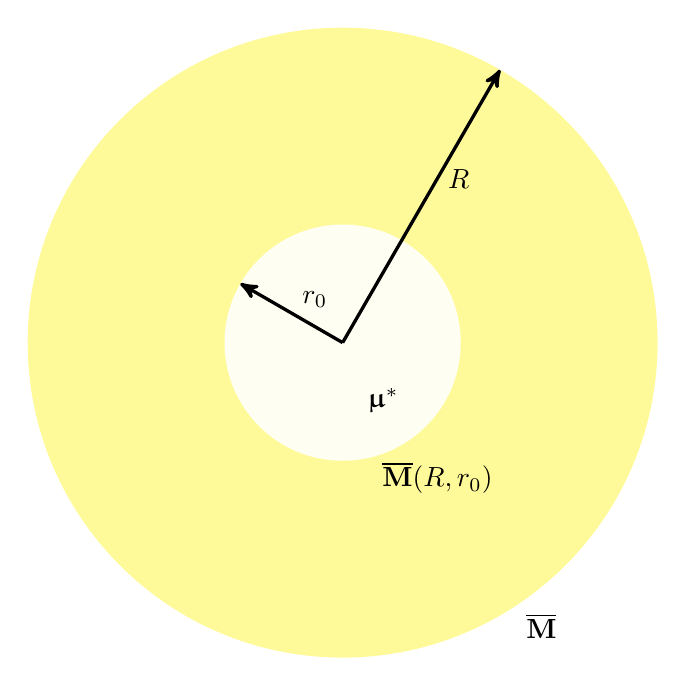
\begin{tikzpicture}
  \newcommand{\sz}{1cm}
  \newcommand{\szR}{4.0*\sz}
  \newcommand{\szr}{1.5*\sz}
  \fill[yellow!40!white] (0, 0) circle (\szR);
  \fill[yellow!5!white] (0, 0) circle (\szr);
  \draw[very thick, ->, >=stealth'] (0, 0) -- (60:\szR)
    node[pos=0.6, anchor=west]{$R$};
  \draw[very thick, ->, >=stealth'] (0, 0) -- (150:\szr)
    node[pos=0.5, anchor=210]{$r_0$};
  \node[] at (-55:0.6*\szr) {$\vmu^*$};
  \node[] at (-55:1.4*\szr) {$\vMbar(R, r_0)$};
  \node[] at (-55:1.1*\szR) {$\vMbar$};
\end{tikzpicture}
\end{center}



\subsection{Eq. (25) and the Green's theorem}



The Green's theorem mentioned before Eq. (25) is the following.
%
For a scale field $\psi$,
an integral over a region $v$
is equal to that over its surface $\vct S$:
\begin{equation}
  \int_v \nabla \psi \, d v
=
  \int_S \psi \, d\vct S,
  \label{eq:green}
\end{equation}
%
where the area element $d\vct S$
assumes the direction of the normal
and points out of the region.

The proof is the following (\cite{arfken}, chapter 1, \S 1.11).
%
The usual Gauss theorem states that
for a vector field $\vct F$,
\begin{equation}
  \int_v \nabla \cdot \vct F \, dv
=
  \int_S \vct F \vct \, d\vct S.
\end{equation}
%
Now let us use $\vct F = \psi \, \vct a$,
Since
\[
  \partial_i (a_i \psi)
= a_i \, \partial_i \psi
\]
we get that
\[
  \vct a \cdot \int_v \nabla \psi \, dv
=
  \vct a \int_S \vct F \vct \, d\vct S.
\]
Since $\vct a$ is arbitrary,
we get Eq. \eqref{eq:green}.

Applying this theorem to $\psi = -(\epsilon - 1) \, \psi_i$,
with the region between the two spheres
of radii $r_0$ and $R$,
we get
\begin{equation}
  \int_{v_0}^v \vP \, dv
=
  -\frac{\epsilon - 1}{4 \pi}
  \int^{S_e} \psi_i \, d\vct S
  +\frac{\epsilon - 1}{4 \pi}
  \int^{S_0} \psi_i \, d\vct S.
\end{equation}
Note,
\[
  4 \pi \, \vP
= (\epsilon - 1) \, \vE
= -(\epsilon - 1) \, \nabla \psi_i,
\]
in Gaussian units.



\subsection{Eq. (27)}



Equation (27) describes a uniform field within the $R$ ball.
\begin{equation}
  \chi
=
  \sum_{n = 1}^\infty
  \sum_{m = -n}^n
  B_{nm} r^n P_n^m(\cos\vartheta)e^{im \varphi}.
  \tag{27}
\end{equation}
%
Assuming that the dipole is along the $z$ axis,
this can be simplified using Legendre polynomials ($m = 0$) only
%
\begin{equation}
  \chi
=
  \sum_{n = 1}^\infty
  B_{n0} r^n P_n(\cos\vartheta).
  \tag{$27'$}
\end{equation}
%
In fact we will only need the $z = 1$ term,
\begin{equation}
  \chi
=
B_{10} \, r \cos\vartheta
=
B_{10} \, z,
  \tag{$27''$}
\end{equation}
%
which represents a uniform field within the $R$ ball.



\subsection{Eq. (28)}



The $\epsilon$ on the left-hand side of Eq. (28)
should be dropped:
\begin{align}
  -\vct\upmu^*\cdot
  \nabla
  \left(
    \frac { 1 }
    { |\vr - \vr'| }
  \right)
&=
  \sum_{n = 0}^\infty
  \sum_{m = -n}^{+n}
  \frac { ( n - |m| )! } { ( n + |m| )! }
  \notag
  \\
&\hphantom{=}\times
  \frac { A_{nm} } { r^{n + 1} }
  P_n^m(\cos\vartheta) e^{im \varphi}.
  \tag{28}
\end{align}
%
Again, if we can simplify this expression
by assuming that $\vmu^*$ aligns on the $z$ axis
$\vr' = \vct 0$, and keep the only relevant $n = 1$ term.
%
\begin{align}
  -\vct\upmu^*\cdot
  \nabla
  \left(
    \frac { 1 }
    { r }
  \right)
&=
  \frac { A_{10} } { r^2 }
  \cos\vartheta
=
  \frac { \mu_z^* } { r^2 }
  \cos\vartheta.
  \tag{$28''$}
\end{align}
%
A possible reason that Kirkwood use
of associated Legendre polynomial
is that he might wish to study a dipole
that does not sit at the symmetric position of the origin.



\subsection{Eq. (30)}



Equations (30),
\begin{equation}
\begin{split}
  M_{nm}
&=
  \frac{ 2 n + 1 } { n \epsilon + n + 1 } A_{nm},
\\
  B_{nm}
&=
  \frac{ n + 1 }{ \epsilon R^{2 n + 1} }
  \frac{ \epsilon - 1 } { n \epsilon \epsilon + n + 1 }
  A_{nm}.
\end{split}
  \tag{30}
\end{equation}
%
are derived from the radial continuity of $\vct D$,
%
\begin{align*}
  \epsilon
  \left(
    \frac { n + 1 }{ \epsilon }
    \frac { A_{nm} } { R^{n+2} }
  - n B_{nm} R^{n - 1}
  \right)
=
  (n + 1) \frac{ M_{nm} }{ R^{n+2} },
\end{align*}
and the tangential continuity of $\vct E$,
\begin{align*}
  \frac { 1 }{ \epsilon }
  \frac { A_{nm} } { R^{n+1} }
+
  B_{nm} R^n
=
  \frac{ M_{nm} }{ R^{n+1} }.
\end{align*}



\subsection{Eq. (33)}



The term $\epsilon - 1$ in Eq. (33) misses a square sign.
\begin{align}
\vMbar
=
\vMbar(R, r_0)
-
\frac{2}{3\epsilon}
\frac{(\epsilon - 1)^2}{\epsilon + 2}
\vct\upmu^*
+ O\left( \frac{ r_0^3 } { R^3 } \right).
\tag{33}
\end{align}



\subsection{Definition of two dipole moments}



Both $\vmu^*$ and $\vMbar(R, r_0)$
Have the meaning of the total dipole of the region $v_0$
(within the sphere of the radius $r_0$).
%
However, from Eqs. (31) and (34), we get
\begin{equation}
  \vmu^* = \frac { 3 \epsilon } { 2 \epsilon + 1 }
  \vMbar(R, r_0) \ne \vMbar(R, r_0).
\end{equation}

It is should be noted that
$\vmu^*$ is simply the parameter
$A_{10}$ in (28)
and thus is not the physical dipole moment.
%
This is the parameter
that makes the region $v_0$
look like an effective dipole
immersed in the media of dielectric constant $\epsilon$.

Thus,
$\vmu^*$
contains some contribution of the polarization of the out sphere.
In fact
\begin{align*}
  \frac{ \vmu^* } { \epsilon }
&=
  \vMbar(R, r_0)
  -
  \frac { 2 (\epsilon - 1) } { 2 \epsilon + 1 } \vMbar(R, r_0).
  \\
&=
  \vMbar(R, r_0)
  -
  B_{10} R^3 \frac{ \epsilon + 2 }{ 3 }.
\end{align*}


\bibliography{../../liquid}
\bibliographystyle{alpha}
\end{document}
